\documentclass[aspectratio=169,10pt]{beamer}
\usetheme{Madrid}
\usecolortheme{seahorse}

\usepackage{amsmath,amssymb,amsfonts}
\usepackage{mathtools}
\usepackage{graphicx}
\usepackage{booktabs}
\usepackage{listings}
\usepackage{xcolor}
\usepackage{tikz}
\usepackage{array}
\usepackage{multirow}
\usepackage{algorithm}
\usepackage{algpseudocode}
\usepackage{hyperref}

\graphicspath{{figures/}}

\definecolor{codebg}{rgb}{0.97,0.97,0.97}
\definecolor{codegreen}{rgb}{0.0,0.5,0.0}
\definecolor{codekw}{rgb}{0.13,0.29,0.53}
\definecolor{codestr}{rgb}{0.73,0.13,0.13}

\lstdefinestyle{pystyle}{
  language=Python,
  basicstyle=\ttfamily\scriptsize,
  keywordstyle=\color{codekw}\bfseries,
  stringstyle=\color{codestr},
  commentstyle=\color{codegreen}\itshape,
  numbers=left,
  numberstyle=\tiny\color{gray},
  stepnumber=1,
  numbersep=5pt,
  frame=single,
  backgroundcolor=\color{codebg},
  breaklines=true,
  showstringspaces=false,
  tabsize=4,
  captionpos=b,
  xleftmargin=12pt,
  xrightmargin=4pt,
}

\setbeamertemplate{footline}[frame number]
\setbeamertemplate{navigation symbols}{}

% ─── Title ────────────────────────────────────────────────────
\title[Discrete Optimization]{Chapter 22: Discrete Optimization}
\subtitle{Algorithms for Optimization, 2nd ed.\ (2026)\\
  \small Kochenderfer \& Wheeler}
\author{Lecture Notes}
\date{2026}

% ─── Convenience macros ───────────────────────────────────────
\newcommand{\bx}{\mathbf{x}}
\newcommand{\bc}{\mathbf{c}}
\newcommand{\bb}{\mathbf{b}}
\newcommand{\bA}{\mathbf{A}}
\newcommand{\bs}{\mathbf{s}}
\newcommand{\bd}{\mathbf{d}}
\newcommand{\bz}{\mathbf{z}}
\newcommand{\RR}{\mathbb{R}}
\newcommand{\ZZ}{\mathbb{Z}}
\newcommand{\NN}{\mathbb{N}}

% ══════════════════════════════════════════════════════════════
\begin{document}
% ══════════════════════════════════════════════════════════════

\begin{frame}
  \titlepage
\end{frame}

%─── Table of Contents ────────────────────────────────────────
\begin{frame}{Chapter Outline}
  \tableofcontents
\end{frame}

% ══════════════════════════════════════════════════════════════
\section{Introduction}
% ══════════════════════════════════════════════════════════════

\begin{frame}{What is Discrete Optimization?}
  \begin{columns}
    \begin{column}{0.55\textwidth}
      \begin{itemize}
        \item Previous chapters: design variables are \textbf{continuous}
        \item Many real problems have \textbf{naturally discrete} variables:
          \begin{itemize}
            \item Manufacturing: number of components
            \item Scheduling: job assignment
            \item Network routing: path selection
          \end{itemize}
        \item Design variables chosen from a \textbf{discrete (finite) set}
        \item Cannot generally use gradient-based methods
        \item Methods covered: rounding, cutting planes, branch \& bound,
              dynamic programming, ant colony optimization
      \end{itemize}
    \end{column}
    \begin{column}{0.43\textwidth}
      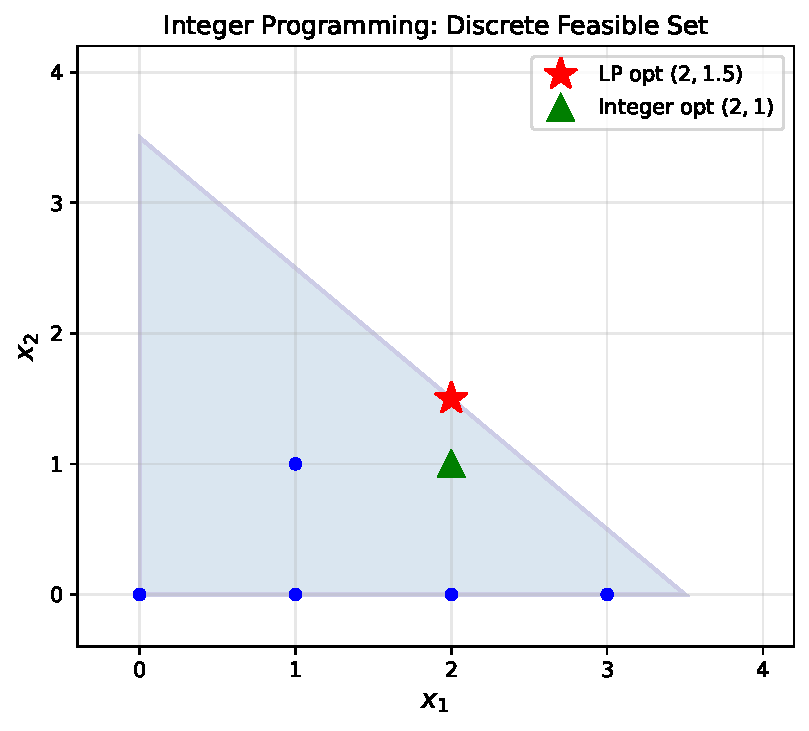
\includegraphics[width=\textwidth]{intro_integer.pdf}
      \vspace{1pt}
      \footnotesize{Discrete feasible points (blue dots) vs.\ LP relaxation
        (red star) and integer optimum (green triangle).}
    \end{column}
  \end{columns}
\end{frame}

% ══════════════════════════════════════════════════════════════
\section{Integer Programs}
% ══════════════════════════════════════════════════════════════

\begin{frame}{Integer Programs --- Standard Form}
  \begin{block}{Definition (Integer Program)}
    An \textbf{integer program (IP)} is a linear program with integral
    constraints on design variables.  Standard (inequality) form:
    \begin{equation}
      \begin{aligned}
        \underset{\bx}{\text{minimize}} \quad & \bc^\top \bx \\
        \text{subject to} \quad & \bA\bx \leq \bb \\
                                & \bx \geq \mathbf{0} \\
                                & \bx \in \ZZ^n
      \end{aligned}
      \tag{22.1}
    \end{equation}
    where $\ZZ^n$ is the set of $n$-dimensional integral vectors,
    $\bc \in \RR^n$, $\bA \in \RR^{m \times n}$, $\bb \in \RR^m$.
  \end{block}

  \begin{itemize}
    \item Also called \emph{integer linear programs} (ILPs)
    \item Modern solvers (Gurobi, CPLEX) handle millions of variables
  \end{itemize}
\end{frame}

\begin{frame}{Equality Form and Mixed-Integer Programs}
  \begin{columns}
    \begin{column}{0.48\textwidth}
      \begin{block}{Equality Form (22.2)}
        \[
          \begin{aligned}
            \underset{\bx,\bs}{\min} & \quad \bc^\top\bx \\
            \text{s.t.} & \quad \bA\bx + \bs = \bb \\
                        & \quad \bx \geq \mathbf{0},\; \bs \geq \mathbf{0} \\
                        & \quad \bx \in \ZZ^n
          \end{aligned}
        \]
        Slack variables $\bs$ need \emph{not} be integral.
      \end{block}
    \end{column}
    \begin{column}{0.50\textwidth}
      \begin{block}{Mixed-Integer Program (22.3)}
        \[
          \begin{aligned}
            \underset{\bx}{\min} & \quad \bc^\top\bx \\
            \text{s.t.} & \quad \bA\bx = \bb \\
                        & \quad \bx \geq \mathbf{0} \\
                        & \quad \bx_{\mathcal{D}} \in \ZZ^{|\mathcal{D}|}
          \end{aligned}
        \]
        $\mathcal{D}$: index set of discrete variables. \\
        $\bx = [\bx_{\mathcal{D}}, \bx_{\mathcal{C}}]$: discrete + continuous.
      \end{block}
    \end{column}
  \end{columns}
  \vspace{4pt}
  \begin{alertblock}{Key Challenge}
    The integrality constraint makes the feasible set \emph{non-convex} and
    \emph{combinatorially large}. NP-hard in general.
  \end{alertblock}
\end{frame}

\begin{frame}{Totally Unimodular Matrices}
  \begin{columns}
    \begin{column}{0.55\textwidth}
      \begin{block}{Definition}
        A matrix $\bA$ is \textbf{totally unimodular (TU)} if every square
        submatrix has determinant $\in \{-1, 0, 1\}$.
      \end{block}
      \begin{itemize}
        \item If $\bA$ is TU and $\bb \in \ZZ^m$, then all LP optimal
              vertices are \textbf{automatically integral}
        \item The LP relaxation solves the IP exactly!
        \item Example: network flow constraint matrices are TU
        \item Single-entry (0/1) matrices with at most one 1 per column
              that appear in bi-partite graphs are TU
      \end{itemize}
    \end{column}
    \begin{column}{0.43\textwidth}
      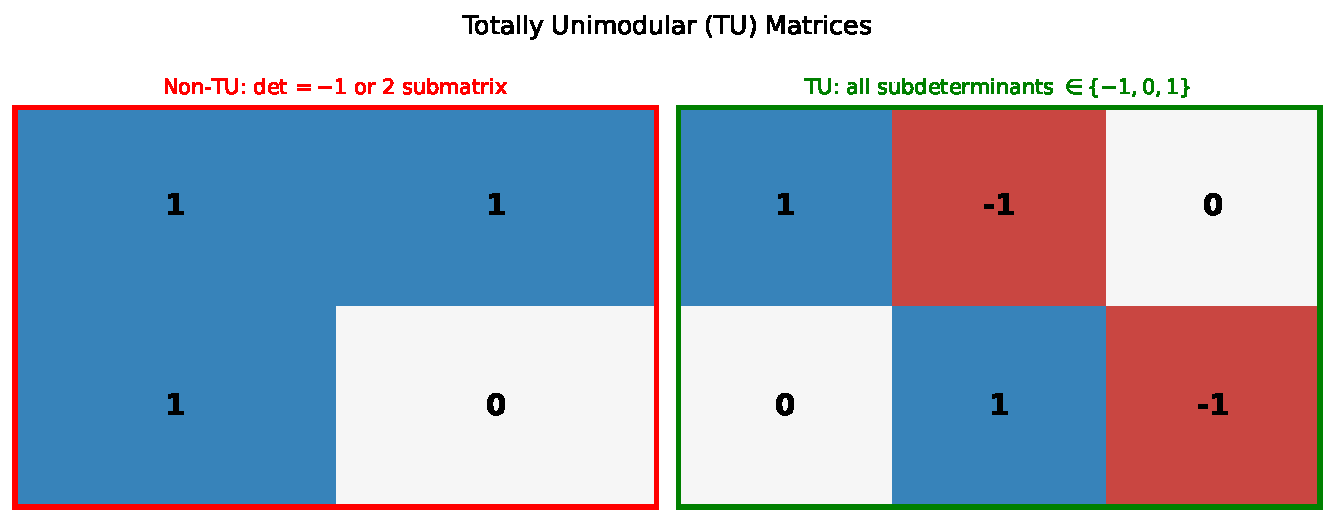
\includegraphics[width=\textwidth]{total_unimodular.pdf}
    \end{column}
  \end{columns}
\end{frame}

% ══════════════════════════════════════════════════════════════
\section{Rounding (LP Relaxation)}
% ══════════════════════════════════════════════════════════════

\begin{frame}{LP Relaxation and Rounding}
  \begin{columns}
    \begin{column}{0.55\textwidth}
      \begin{block}{LP Relaxation}
        Drop the integrality constraint $\bx \in \ZZ^n$ and solve the
        resulting LP. This gives a \textbf{lower bound} on the IP optimum.
      \end{block}

      \textbf{Rounding strategies:}
      \begin{enumerate}
        \item \textbf{Simple floor/ceiling:} $\hat{x}_i = \lfloor x^*_i \rfloor$
              or $\lceil x^*_i \rceil$ \\
              \emph{Problem: may be infeasible!}
        \item \textbf{Probabilistic rounding:} round $x^*_i$ up with
              probability equal to its fractional part
        \item \textbf{Iterative rounding:} fix most-rounded component,
              re-solve
      \end{enumerate}
      \vspace{4pt}
      \begin{alertblock}{Caveat}
        For some problems, rounding yields a solution that is far from
        optimal or \emph{infeasible}.
      \end{alertblock}
    \end{column}
    \begin{column}{0.43\textwidth}
      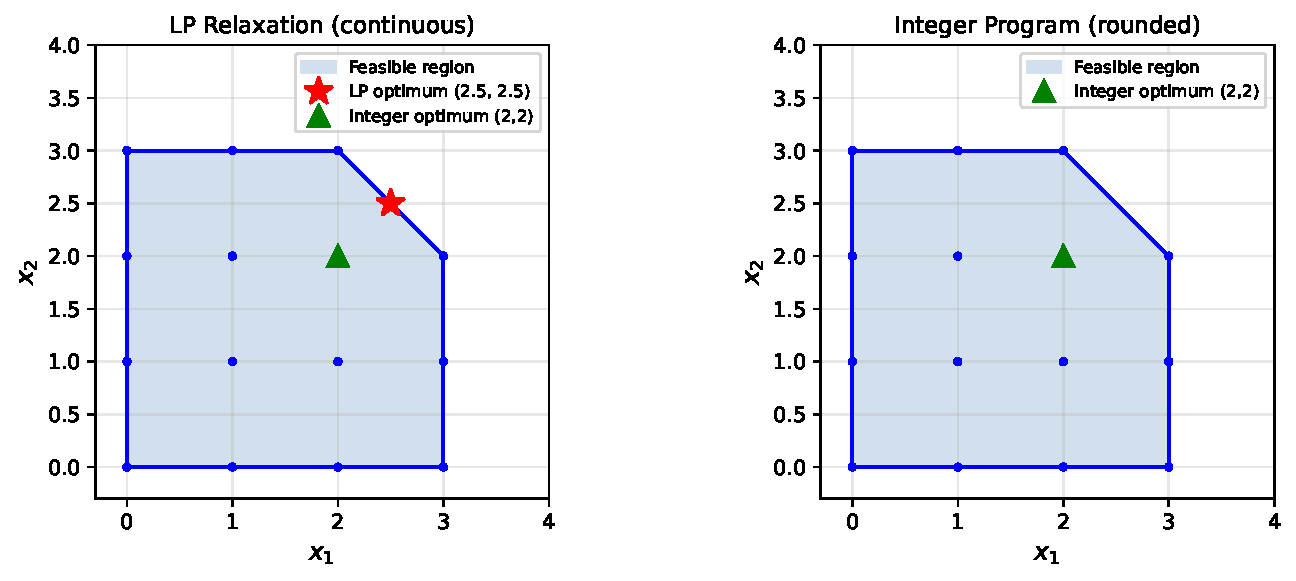
\includegraphics[width=\textwidth]{lp_relaxation.pdf}
      \vspace{2pt}
      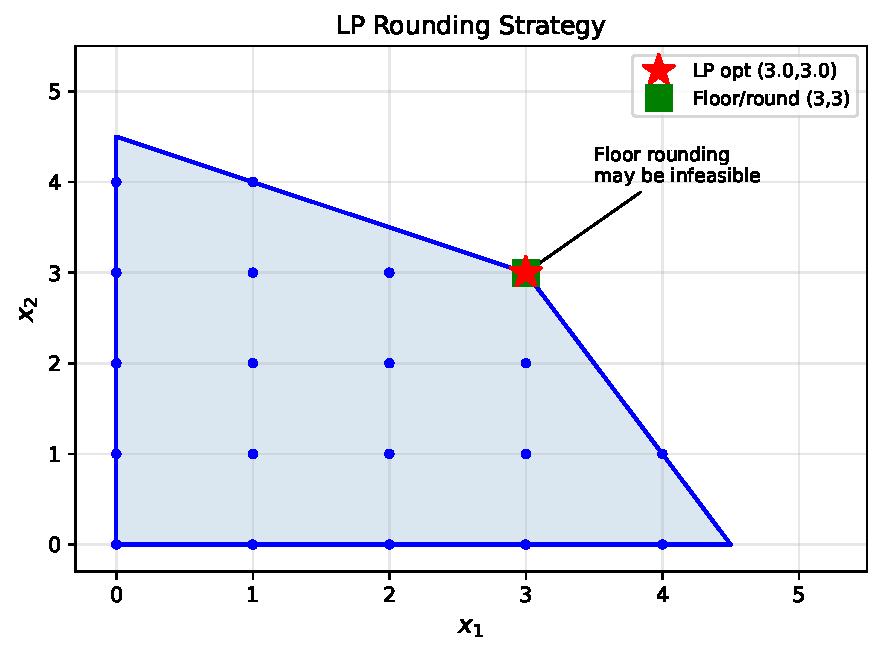
\includegraphics[width=\textwidth]{rounding.pdf}
    \end{column}
  \end{columns}
\end{frame}

\begin{frame}[fragile]{Rounding --- Python Example}
\begin{lstlisting}[style=pystyle, caption={LP relaxation + rounding with scipy}]
import numpy as np
from scipy.optimize import linprog

# Integer program:  minimize  c @ x
#   subject to      A_ub @ x <= b_ub
#                   x >= 0,  x in Z^n
c     = np.array([1.0, 2.0])       # objective
A_ub  = np.array([[-1.0, -1.0],    # -x1 - x2 <= -3  (i.e. x1+x2>=3)
                  [ 1.0,  2.0]])   #  x1 + 2x2 <= 7
b_ub  = np.array([-3.0, 7.0])
bounds = [(0, None), (0, None)]

# Step 1: solve LP relaxation
res = linprog(c, A_ub=A_ub, b_ub=b_ub, bounds=bounds, method='highs')
x_lp = res.x
print(f"LP relaxation: x = {x_lp}, obj = {res.fun:.4f}")

# Step 2: simple rounding (floor)
x_floor = np.floor(x_lp).astype(int)
x_ceil  = np.ceil(x_lp).astype(int)
print(f"Floor rounded: {x_floor}, obj = {c @ x_floor:.4f}")
print(f"Ceil  rounded: {x_ceil},  obj = {c @ x_ceil:.4f}")

# Step 3: check feasibility of rounded solutions
for name, xr in [('floor', x_floor), ('ceil', x_ceil)]:
    feasible = np.all(A_ub @ xr <= b_ub + 1e-8)
    print(f"{name}: feasible = {feasible}")
\end{lstlisting}
\end{frame}

% ══════════════════════════════════════════════════════════════
\section{Cutting Planes (Gomory Cuts)}
% ══════════════════════════════════════════════════════════════

\begin{frame}{Cutting Plane Method}
  \begin{columns}
    \begin{column}{0.55\textwidth}
      \textbf{Idea:} iteratively add \emph{valid cuts} (linear inequalities)
      that eliminate the current fractional LP optimum while not removing
      any integer-feasible point.

      \vspace{4pt}
      \textbf{Procedure:}
      \begin{enumerate}
        \item Solve the LP relaxation; get solution $\bx^*$
        \item If $\bx^*$ is integral, we are done
        \item Find a cutting plane that:
              (a) cuts off $\bx^*$, and
              (b) is satisfied by all integer-feasible points
        \item Add the cut to the LP, go to step 1
      \end{enumerate}
      \vspace{4pt}
      Each iteration \textbf{tightens} the LP relaxation, moving the LP
      optimum toward an integer solution.
    \end{column}
    \begin{column}{0.43\textwidth}
      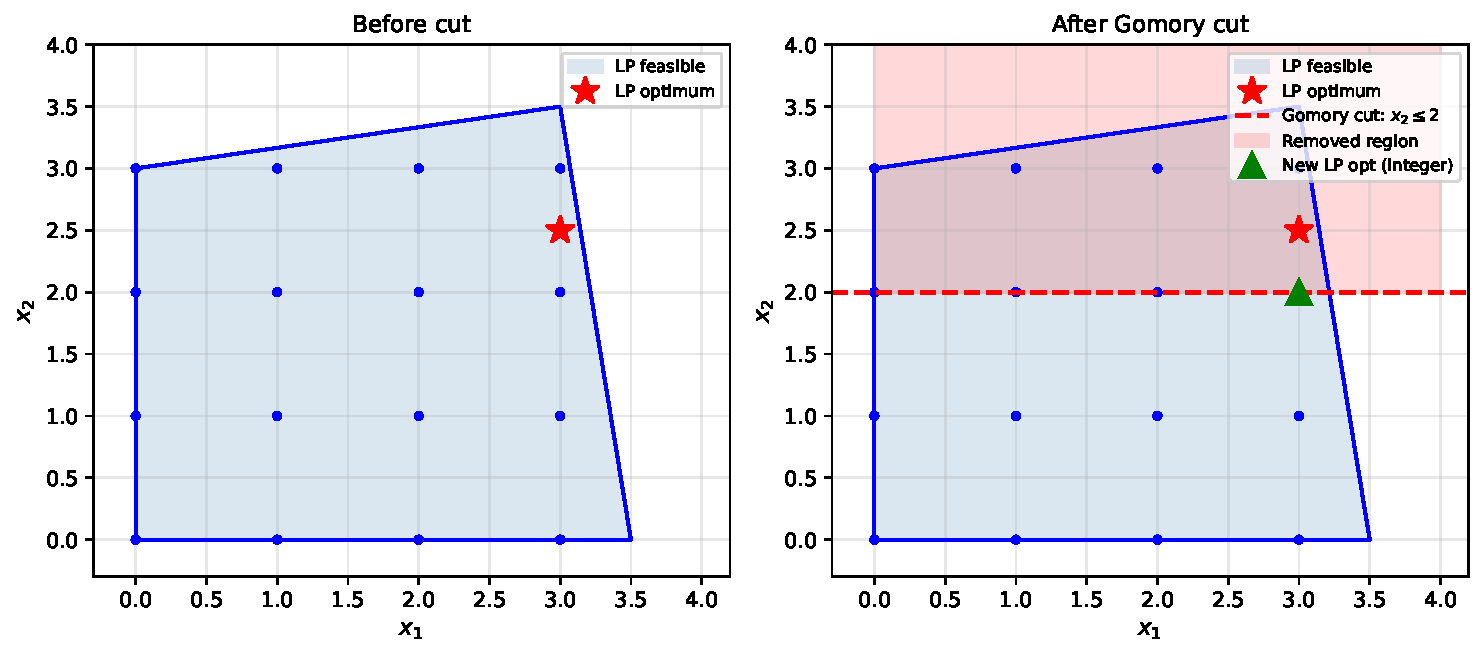
\includegraphics[width=\textwidth]{cutting_planes.pdf}
      \vspace{2pt}
      \footnotesize{Left: LP optimum is fractional. Right: after adding
        a Gomory cut, the LP optimum is integer-valued.}
    \end{column}
  \end{columns}
\end{frame}

\begin{frame}{Gomory Cuts --- Derivation}
  \begin{block}{Gomory Cut (Eq.\ 22.10--22.11)}
    Given a non-integral LP optimal solution $\bx^*$ (basis $B$), for a
    non-integral basic variable $x_i$ with $\bar{x}_i \notin \ZZ$:
    \begin{equation}
      x_i + \sum_{j \notin B} \bigl(\lfloor\bar{A}_{ij}\rfloor
        - \bar{A}_{ij}\bigr)\,x_j
      \;\leq\; \lfloor\bar{b}_i\rfloor
      \tag{22.11}
    \end{equation}
    where $\bar{\bA} = \bA_B^{-1}\bA_V$ and $\bar{\bb} = \bA_B^{-1}\bb$.
  \end{block}

  \textbf{Symbols:}
  \begin{itemize}
    \item $B$: set of basic variable indices; $\bA_B$: basic submatrix
    \item $V$: set of non-basic (variable) indices
    \item $\bar{A}_{ij}$: $(i,j)$ entry of the reduced basis matrix
    \item $\lfloor \cdot \rfloor$: floor function; $\text{frac}(x) = x - \lfloor x \rfloor$
  \end{itemize}

  \begin{block}{Key Property}
    The cut is \emph{valid}: all integer-feasible points satisfy it.
    It is \emph{tight}: the current LP solution violates it.
  \end{block}
\end{frame}

\begin{frame}{Gomory Cut --- Running Example (Ex.\ 22.3)}
  \begin{block}{Problem}
    \[
      \underset{\bx}{\text{minimize}}\; 2x_1 + x_2 + 3x_3
      \quad\text{s.t.}\quad
      \begin{bmatrix}0.5 & -0.5 & 1.0 \\ 2.0 & 0.5 & -1.5\end{bmatrix}\bx
      = \begin{bmatrix}2.5\\-1.5\end{bmatrix},
      \;\bx \geq \mathbf{0},\;\bx \in \ZZ^3
    \]
  \end{block}

  \textbf{Iteration 1:} LP relaxation gives $\bx^* \approx [0.818, 0, 2.091]$
  (non-integral). Gomory cuts derived:
  \[
    x_4 - 0.909\,x_2 = -0.818
    \qquad
    x_5 - 0.545\,x_2 = -0.091
  \]

  \textbf{Iteration 2:} Solve augmented LP $\Rightarrow$
  $\bx^* \approx [0.9, 0.9, 2.5, 0.0, 0.4]$. Still fractional.
  Add more cuts.

  \textbf{Iteration 3:} Solve $\Rightarrow$
  $\bx^* = [1, 2, 3, 1, 1, 0, 0, 0, 0]$.
  \textbf{Final solution:} $\bx_i^* = [1, 2, 3]$.

  \vspace{4pt}
  \textit{Complexity:} Each iteration adds one constraint; convergence is
  finite for bounded IPs (Gomory, 1958), but may need exponentially many cuts.
\end{frame}

\begin{frame}[fragile]{Cutting Plane Algorithm --- Python}
\begin{lstlisting}[style=pystyle, caption={Cutting plane method (Gomory) in Python}]
import numpy as np
from scipy.optimize import linprog

def frac(x):
    return x - np.floor(x)

def cutting_plane_ip(c, A_eq, b_eq, n_orig, max_iter=30):
    """Gomory cutting plane for equality-form IP (x >= 0, x in Z^n_orig)."""
    A, b = A_eq.copy(), b_eq.copy()
    c_aug = np.concatenate([c, np.zeros(0)])

    for iteration in range(max_iter):
        # Solve LP relaxation
        res = linprog(c_aug, A_eq=A, b_eq=b,
                      bounds=[(0, None)]*A.shape[1], method='highs')
        if res.status != 0:
            raise ValueError("LP infeasible or unbounded")
        x = res.x

        # Check integrality of original variables
        frac_vals = frac(x[:n_orig])
        if np.all(frac_vals < 1e-6):
            return np.round(x[:n_orig]).astype(int)

        # Find most fractional variable
        i = np.argmax(frac_vals)
        fi = frac_vals[i]
        # Gomory cut: add slack s >= 0, coefficient row
        # (simplified: use the basis row for variable i)
        n_vars = A.shape[1]
        cut_row = np.zeros(n_vars + 1)
        cut_row[i] = 1.0           # simplified cut
        cut_row[-1] = 1.0          # slack variable
        cut_rhs = np.floor(x[i])

        A = np.block([[A, np.zeros((A.shape[0], 1))],
                      [cut_row.reshape(1, -1)]])
        b = np.append(b, cut_rhs)
        c_aug = np.append(c_aug, 0.0)

    return np.round(x[:n_orig]).astype(int)
\end{lstlisting}
\end{frame}

% ══════════════════════════════════════════════════════════════
\section{Branch and Bound}
% ══════════════════════════════════════════════════════════════

\begin{frame}{Branch and Bound --- Overview}
  \begin{columns}
    \begin{column}{0.55\textwidth}
      \begin{block}{Idea}
        Enumerate solutions implicitly by \emph{branching} on a fractional
        variable and maintaining \emph{bounds} to prune the search tree.
      \end{block}

      \textbf{Three operations:}
      \begin{enumerate}
        \item \textbf{Branch:} split on a non-integral component $x_{i}^*$
              into two sub-LPs:
              $x_i \leq \lfloor x_i^*\rfloor$ and
              $x_i \geq \lceil x_i^*\rceil$
        \item \textbf{Bound:} solve LP relaxation of each child to get a
              lower bound $y \geq \bc^\top\bx^*$
        \item \textbf{Prune:} discard branches where the lower bound
              exceeds the current best integer solution (\emph{incumbent})
      \end{enumerate}

      \textbf{Priority:} use a priority queue ordered by LP bound;
      explore the most promising node first.
    \end{column}
    \begin{column}{0.43\textwidth}
      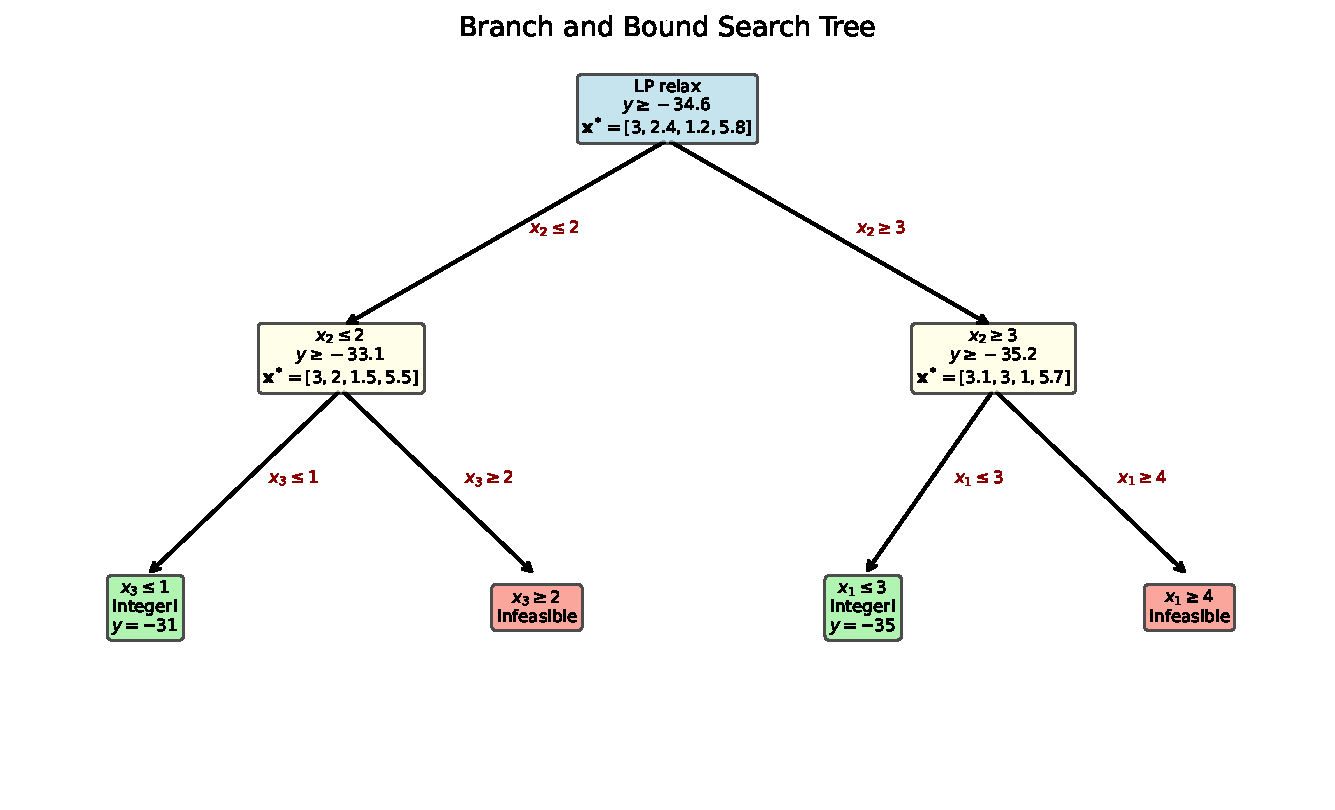
\includegraphics[width=\textwidth]{branch_bound_tree.pdf}
    \end{column}
  \end{columns}
\end{frame}

\begin{frame}{Branching Splits the Feasible Set (Fig.\ 22.4)}
  \begin{center}
    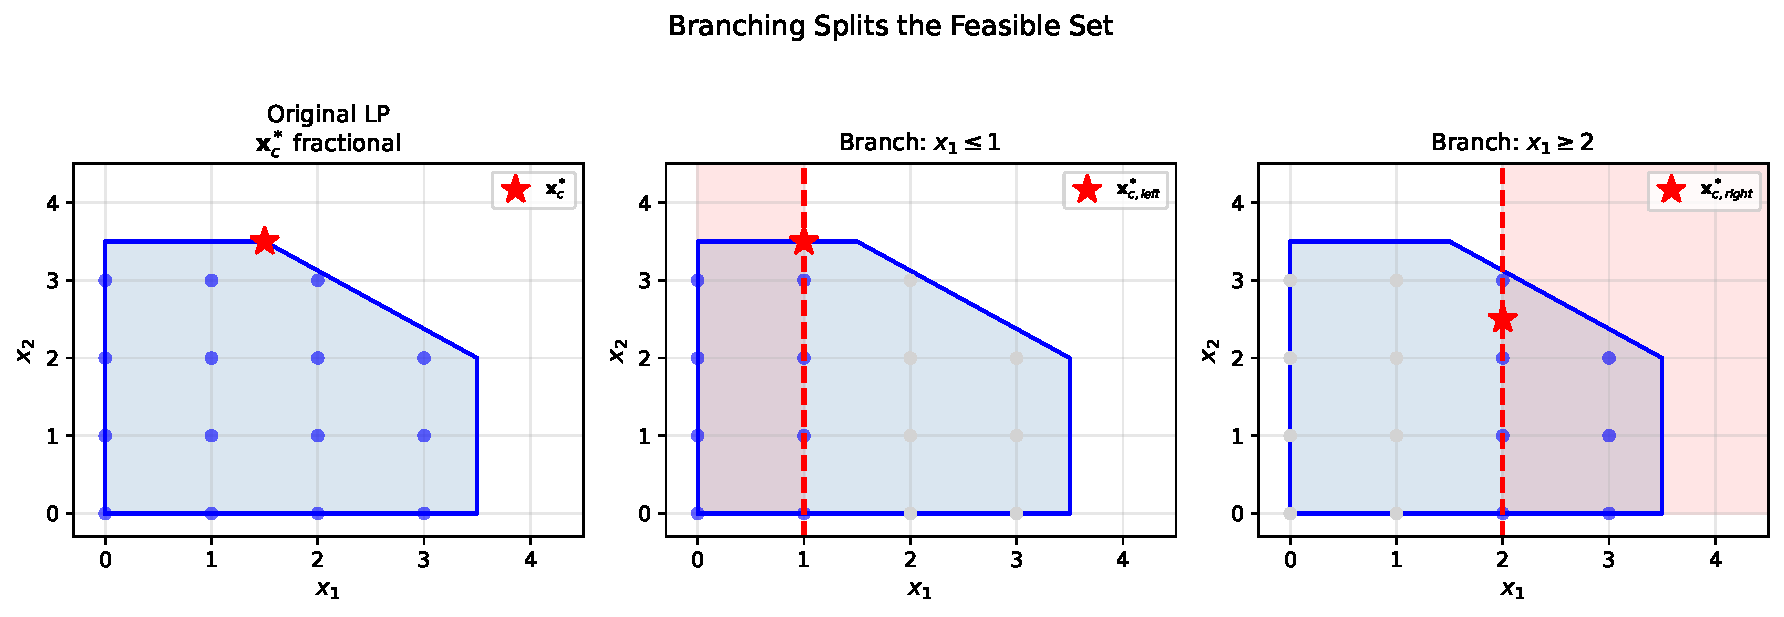
\includegraphics[width=0.92\textwidth]{branching_split.pdf}
  \end{center}
  \footnotesize
  When $x_1^* = 1.5$ (fractional), we split into two sub-problems:
  $x_1 \leq 1$ (left) and $x_1 \geq 2$ (right).
  Each sub-problem has fewer feasible integer points.
\end{frame}

\begin{frame}{Branch and Bound --- Branching Example (Ex.\ 22.4)}
  \begin{block}{Setup}
    LP relaxation gives $\bx^*_c = [3, 2.4, 1.2, 5.8]$ with
    $\bc = [-1,-2,-3,-4]$.  Lower bound: $y \geq \bc^\top\bx^*_c = -34.6$.
  \end{block}

  \textbf{Branching step:}
  \begin{itemize}
    \item Choose the non-integral component farthest from an integer:
          $x_{2,c}^* = 2.4$ (distance $0.4$ from 2 or 3)
    \item Create two sub-problems:
      \begin{itemize}
        \item \textbf{Left:} add $x_2 \leq 2$
        \item \textbf{Right:} add $x_2 \geq 3$
      \end{itemize}
    \item Solve each sub-LP to get new lower bounds
    \item Keep expanding the most promising leaf
  \end{itemize}

  \begin{alertblock}{Pruning Conditions}
    A node is pruned if:
    (a) LP is infeasible,
    (b) LP bound $\geq$ current best integer objective,
    (c) LP solution is already integral.
  \end{alertblock}
\end{frame}

\begin{frame}[fragile]{Branch and Bound --- Python Implementation}
\begin{lstlisting}[style=pystyle, caption={Branch and bound for mixed-integer programs}]
import numpy as np
from scipy.optimize import linprog
import heapq

def branch_and_bound(c, A_ub, b_ub, int_vars, bounds=None):
    """Branch and bound for minimization IP.
       int_vars: list of indices that must be integer."""
    n = len(c)
    if bounds is None:
        bounds = [(0, None)] * n
    best_val = np.inf
    best_x   = None
    # Priority queue: (LP_bound, id, A_ub, b_ub, bounds)
    counter  = [0]
    def push(A, b, bds):
        res = linprog(c, A_ub=A, b_ub=b, bounds=bds, method='highs')
        if res.status == 0:
            heapq.heappush(pq, (res.fun, counter[0], A, b, bds, res.x))
            counter[0] += 1
    pq = []
    push(A_ub, b_ub, bounds)
    while pq:
        lb, _, A, b, bds, x = heapq.heappop(pq)
        if lb >= best_val:          # prune: bound exceeds incumbent
            continue
        frac = {i: x[i] - np.floor(x[i]) for i in int_vars
                if abs(x[i] - round(x[i])) > 1e-6}
        if not frac:                # all integer variables are integral
            if lb < best_val:
                best_val, best_x = lb, x.copy()
            continue
        i = max(frac, key=frac.get) # branch on most fractional variable
        # Left branch: x[i] <= floor(x[i])
        row_l = np.zeros(n); row_l[i] = 1.0
        push(np.vstack([A, row_l]), np.append(b, np.floor(x[i])), bds)
        # Right branch: x[i] >= ceil(x[i])
        row_r = np.zeros(n); row_r[i] = -1.0
        push(np.vstack([A, row_r]), np.append(b, -np.ceil(x[i])),  bds)
    return best_x, best_val
\end{lstlisting}
\end{frame}

\begin{frame}{Branch and Bound --- Complexity and Notes}
  \begin{columns}
    \begin{column}{0.55\textwidth}
      \begin{block}{Complexity}
        \begin{itemize}
          \item Worst case: $O(2^n)$ nodes (full binary tree)
          \item In practice: effective pruning makes B\&B much faster
          \item LP solve at each node: $O(m^2 n)$ (simplex)
          \item Total typical: polynomial-ish on structured problems
        \end{itemize}
      \end{block}

      \textbf{Improvements in practice:}
      \begin{itemize}
        \item \textbf{Variable selection:} choose most fractional or
              using pseudo-costs
        \item \textbf{Node selection:} best-first, depth-first, or hybrid
        \item \textbf{Warm starts:} reuse LP basis from parent node
        \item \textbf{Combine} with cutting planes
              (\emph{branch-and-cut}, used in Gurobi/CPLEX)
      \end{itemize}
    \end{column}
    \begin{column}{0.43\textwidth}
      \begin{block}{Example: IP with $n=4$}
        \[
          \bc = [-1,-2,-3,-4]
        \]
        \[
          \bx^*_c = [3,\,2.4,\,1.2,\,5.8]
        \]
        \[
          y \geq -34.6 \text{ (LP bound)}
        \]
        Branch on $x_2$ (farthest from integer).
        \smallskip

        After 3 levels, integer solution found.
      \end{block}
    \end{column}
  \end{columns}
\end{frame}

% ══════════════════════════════════════════════════════════════
\section{Dynamic Programming}
% ══════════════════════════════════════════════════════════════

\begin{frame}{Dynamic Programming for Discrete Optimization}
  \begin{columns}
    \begin{column}{0.55\textwidth}
      \begin{block}{Key Idea}
        Exploit \textbf{optimal substructure}: the optimal solution to a
        large problem can be composed from optimal solutions to smaller
        \emph{overlapping subproblems}.
      \end{block}

      \textbf{Two implementations:}
      \begin{enumerate}
        \item \textbf{Top-down (memoization):} recurse with caching
        \item \textbf{Bottom-up (tabulation):} fill table iteratively
      \end{enumerate}

      \textbf{When applicable:}
      \begin{itemize}
        \item Problem has \emph{optimal substructure}
        \item Subproblems \emph{overlap} (same state visited many times)
        \item State space is \emph{manageable} in size
      \end{itemize}
    \end{column}
    \begin{column}{0.43\textwidth}
      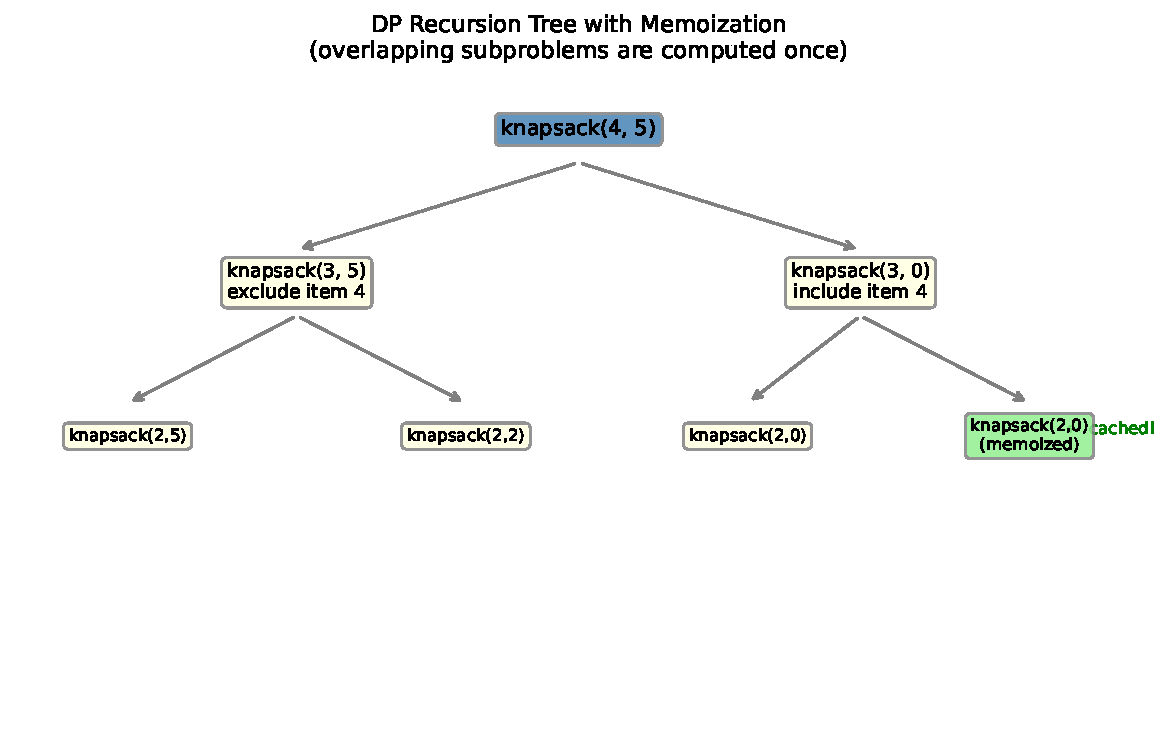
\includegraphics[width=\textwidth]{dp_recursion.pdf}
      \vspace{2pt}
      \footnotesize{Memoized subproblems (green) are computed once and
        cached.}
    \end{column}
  \end{columns}
\end{frame}

\begin{frame}{The 0-1 Knapsack Problem}
  \begin{block}{Problem Formulation (Eq.\ 22.13)}
    Given $n$ items with weights $w_i$ and values $v_i$, and capacity
    $w_{\max}$:
    \[
      \underset{\bx}{\text{minimize}} \;-\sum_{i=1}^n v_i x_i
      \quad\text{s.t.}\quad \sum_{i=1}^n w_i x_i \leq w_{\max},
      \quad x_i \in \{0,1\}
    \]
    $2^n$ possible solutions --- direct enumeration intractable.
  \end{block}

  \begin{block}{DP Recurrence (Eq.\ 22.14)}
    Define $\text{knapsack}(i, w_{\max})$ = max value using items
    $1,\ldots,i$ with capacity $w_{\max}$:
    \[
      \text{knapsack}(i, w_{\max}) =
      \begin{cases}
        0 & i = 0 \\
        \text{knapsack}(i-1, w_{\max}) & w_i > w_{\max} \\
        \max\!\begin{cases}
          \text{knapsack}(i-1, w_{\max}) & \text{(discard)} \\
          \text{knapsack}(i-1, w_{\max}-w_i) + v_i & \text{(include)}
        \end{cases} & \text{otherwise}
      \end{cases}
    \]
  \end{block}
  \textbf{Complexity:} $O(n \cdot w_{\max})$ time and space (pseudo-polynomial).
\end{frame}

\begin{frame}{Knapsack DP Table Visualization}
  \begin{center}
    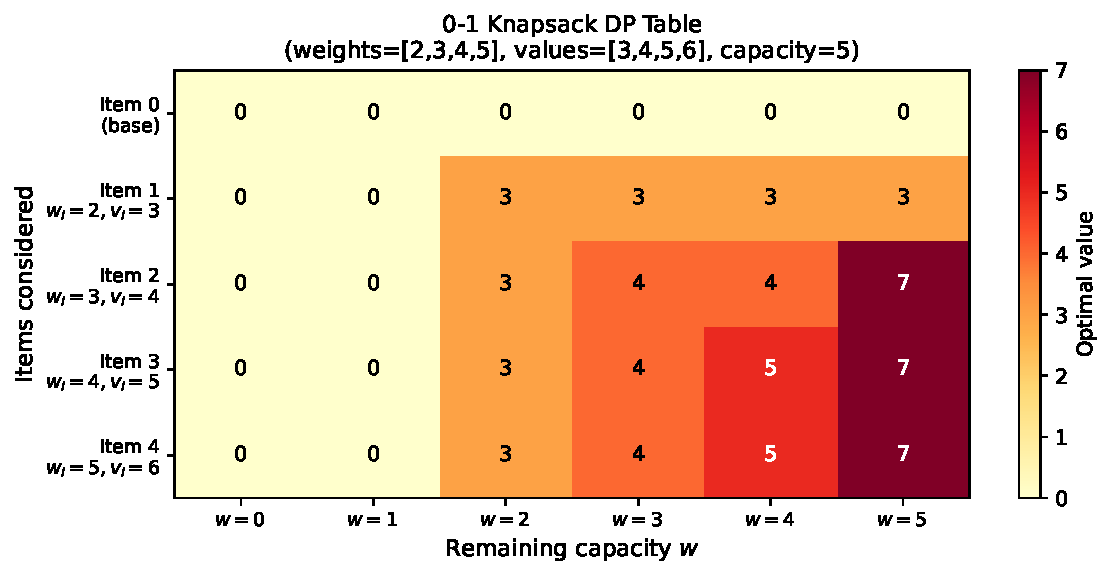
\includegraphics[width=0.85\textwidth]{knapsack_dp.pdf}
  \end{center}
  \footnotesize
  Items: weights $= [2,3,4,5]$, values $= [3,4,5,6]$, capacity $= 5$.
  Each cell shows the maximum value achievable using the first $i$ items
  with remaining capacity $w$.  Optimal value $= 7$ (items 1 and 2).
\end{frame}

\begin{frame}[fragile]{Knapsack DP --- Python Implementation}
\begin{lstlisting}[style=pystyle, caption={0-1 Knapsack via dynamic programming (Python)}]
import numpy as np

def knapsack(weights, values, w_max):
    """0-1 Knapsack via bottom-up DP.
    Returns (max_value, selected_items_mask)."""
    n = len(weights)
    # dp[i][w] = max value with items 0..i-1 and capacity w
    dp = np.zeros((n + 1, w_max + 1), dtype=float)

    for i in range(1, n + 1):
        wi, vi = weights[i-1], values[i-1]
        for w in range(w_max + 1):
            dp[i, w] = dp[i-1, w]           # exclude item i
            if wi <= w:
                dp[i, w] = max(dp[i, w],
                               dp[i-1, w - wi] + vi)  # include item i

    # Traceback to find selected items
    selected = np.zeros(n, dtype=bool)
    w = w_max
    for i in range(n, 0, -1):
        if dp[i, w] != dp[i-1, w]:
            selected[i-1] = True
            w -= weights[i-1]

    return dp[n, w_max], selected

# Example
weights = [2, 3, 4, 5]
values  = [3, 4, 5, 6]
val, sel = knapsack(weights, values, w_max=5)
print(f"Max value: {val}")          # 7
print(f"Selected:  {sel}")          # [True, True, False, False]
print(f"Total weight: {sum(w for w,s in zip(weights,sel) if s)}")  # 5
\end{lstlisting}
\end{frame}

\begin{frame}[fragile]{DP --- Top-Down (Memoized) Implementation}
\begin{lstlisting}[style=pystyle, caption={Top-down memoized knapsack (Python)}]
from functools import lru_cache

def knapsack_topdown(weights, values, w_max):
    """Top-down memoized knapsack."""
    n = len(weights)

    @lru_cache(maxsize=None)
    def dp(i, w):
        """Max value using items i..n-1 with remaining capacity w."""
        if i == n:
            return 0.0
        # Option 1: skip item i
        result = dp(i + 1, w)
        # Option 2: include item i (if it fits)
        if weights[i] <= w:
            result = max(result, values[i] + dp(i + 1, w - weights[i]))
        return result

    return dp(0, w_max)

# Example
weights = [2, 3, 4, 5]
values  = [3, 4, 5, 6]
print(knapsack_topdown(weights, values, w_max=5))  # 7
\end{lstlisting}
\end{frame}

% ══════════════════════════════════════════════════════════════
\section{Ant Colony Optimization}
% ══════════════════════════════════════════════════════════════

\begin{frame}{Ant Colony Optimization --- Motivation}
  \begin{columns}
    \begin{column}{0.55\textwidth}
      \begin{block}{Biological Inspiration}
        Real ants deposit \emph{pheromones} on paths; shorter paths
        accumulate more pheromone over time, attracting more ants ---
        positive feedback reinforces good routes.
      \end{block}

      \textbf{ACO applications:}
      \begin{itemize}
        \item Traveling Salesman Problem (TSP)
        \item Vehicle routing
        \item Network routing (IP packet routing)
        \item Job scheduling
      \end{itemize}

      \textbf{Key components:}
      \begin{itemize}
        \item Pheromone matrix $\tau(i \to j)$
        \item Heuristic (edge attractiveness) $\eta(i \to j)$
        \item Transition probability based on both
        \item Pheromone evaporation $\rho$
      \end{itemize}
    \end{column}
    \begin{column}{0.43\textwidth}
      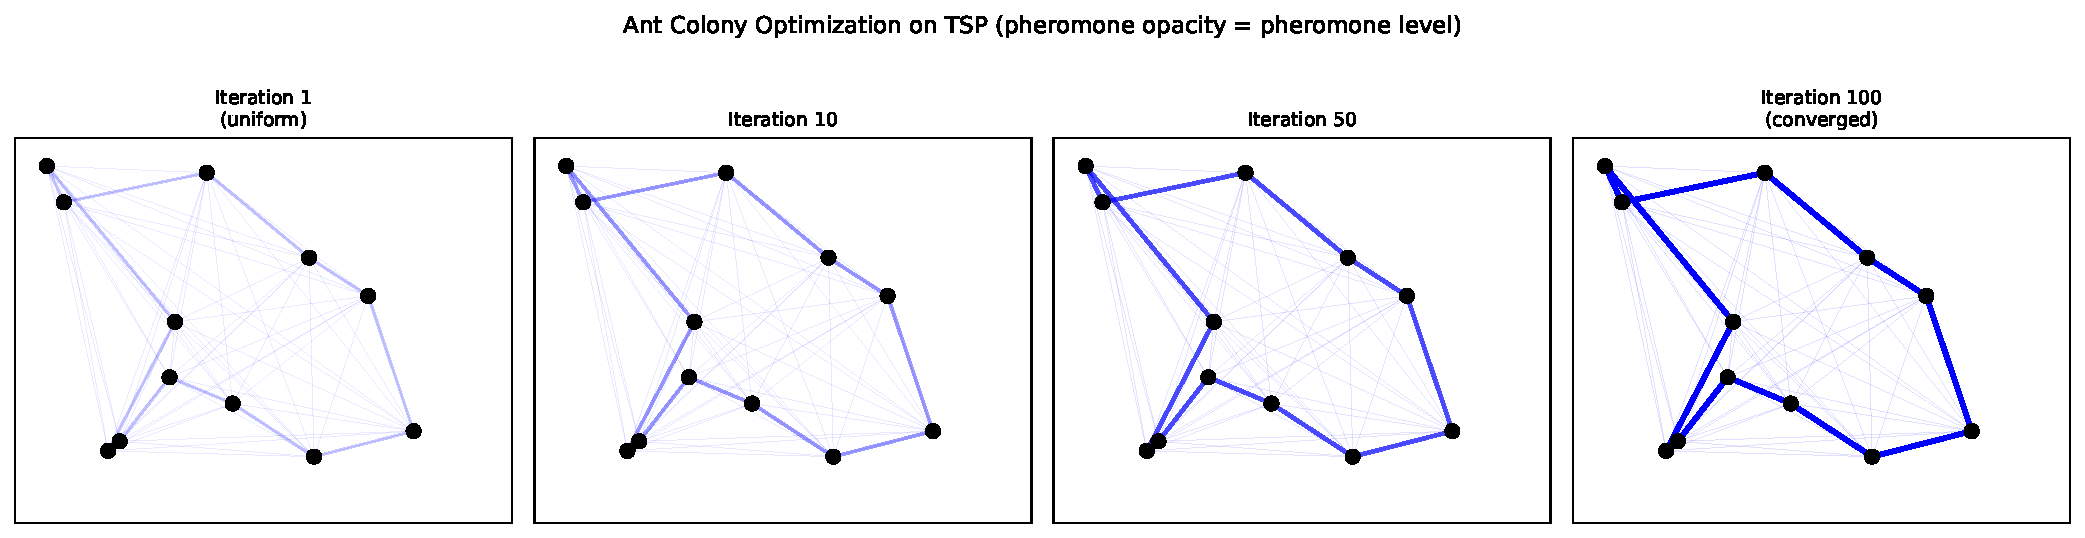
\includegraphics[width=\textwidth]{aco_tsp.pdf}
      \vspace{2pt}
      \footnotesize{ACO on TSP: pheromone level shown by edge opacity.
        Path quality improves with iterations.}
    \end{column}
  \end{columns}
\end{frame}

\begin{frame}{ACO --- Edge Attractiveness and Transition Probability}
  \begin{block}{Edge Attractiveness (Eq.\ 22.15)}
    The attractiveness of edge $(i \to j)$ combines pheromone and prior:
    \[
      A(i \to j) = \tau(i \to j)^\alpha \cdot \eta(i \to j)^\beta
    \]
    where:
    \begin{itemize}
      \item $\tau(i \to j)$: pheromone level on edge $(i \to j)$
      \item $\eta(i \to j) = 1/\text{length}(i \to j)$: heuristic (inverse length)
      \item $\alpha$: pheromone exponent (default 1.0)
      \item $\beta$: prior exponent (default 5.0)
    \end{itemize}
  \end{block}

  \begin{block}{Transition Probability (Eq.\ 22.16)}
    From node $i$ with unvisited neighbors $\mathcal{N}$:
    \[
      P(i \to j) = \frac{A(i \to j)}{\sum_{k \in \mathcal{N}} A(i \to k)}
      \quad \forall j \in \mathcal{N}
    \]
    Ant $a$ samples the next node according to this distribution.
  \end{block}
\end{frame}

\begin{frame}{ACO --- Pheromone Update and Evaporation}
  \begin{block}{Pheromone Update (Eq.\ 22.17)}
    After all $m$ ants complete their tours at iteration $k$:
    \[
      \tau(i \to j)^{(k+1)}
        = (1 - \rho)\,\tau(i \to j)^{(k)}
          + \sum_{a=1}^{m} \frac{1}{\ell^{(a)}}
            \cdot \mathbf{1}\!\bigl[(i \to j) \in \mathcal{P}^{(a)}\bigr]
    \]
    where:
    \begin{itemize}
      \item $\rho \in [0,1]$: evaporation rate (common: $\rho = 0.5$)
      \item $\ell^{(a)}$: total path length of ant $a$'s tour
      \item $\mathcal{P}^{(a)}$: set of edges traversed by ant $a$
      \item $(1-\rho)$: evaporation factor --- prevents premature convergence
    \end{itemize}
  \end{block}

  \begin{alertblock}{Evaporation}
    Without evaporation, early bad paths accumulate pheromone and the
    algorithm gets stuck.  $\rho = 1/2$ is a common default.
  \end{alertblock}
\end{frame}

\begin{frame}[fragile]{ACO --- Python Implementation}
\begin{lstlisting}[style=pystyle, caption={Ant colony optimization for TSP (Python)}]
import numpy as np

def ant_colony_optimization(coords, n_ants=50, n_iter=100,
                             alpha=1.0, beta=5.0, rho=0.5):
    """ACO for TSP. coords: (n,2) array of city positions."""
    n = len(coords)
    # Distance matrix
    dist = np.linalg.norm(coords[:, None] - coords[None, :], axis=2)
    dist[dist == 0] = 1e-10
    eta = 1.0 / dist                        # heuristic
    tau = np.ones((n, n))                   # pheromone (init uniform)

    best_tour, best_len = None, np.inf

    for _ in range(n_iter):
        tours, lengths = [], []
        for ant in range(n_ants):
            visited = [0]
            for step in range(n - 1):
                curr = visited[-1]
                unvisited = [j for j in range(n) if j not in visited]
                # Compute transition probabilities
                attract = np.array([tau[curr,j]**alpha * eta[curr,j]**beta
                                    for j in unvisited])
                probs = attract / attract.sum()
                nxt = unvisited[np.random.choice(len(unvisited), p=probs)]
                visited.append(nxt)
            # Compute tour length (return to start)
            length = sum(dist[visited[i], visited[(i+1)%n]]
                         for i in range(n))
            tours.append(visited); lengths.append(length)
            if length < best_len:
                best_tour, best_len = visited[:], length
        # Pheromone evaporation
        tau *= (1 - rho)
        # Pheromone deposit
        for tour, length in zip(tours, lengths):
            for i in range(n):
                tau[tour[i], tour[(i+1)%n]] += 1.0 / length

    return best_tour, best_len
\end{lstlisting}
\end{frame}

\begin{frame}{ACO Algorithm Summary}
  \begin{columns}
    \begin{column}{0.58\textwidth}
      \textbf{Algorithm (Alg.\ 22.10):}
      \begin{enumerate}
        \item Initialize $\tau(i \to j) = 1$ for all edges
        \item For $k = 1, \ldots, k_{\max}$:
          \begin{enumerate}
            \item Compute edge attractiveness $A(i \to j)$
            \item Apply evaporation: $\tau \leftarrow (1-\rho)\tau$
            \item For each of $m$ ants: simulate tour using
                  transition probabilities (Alg.\ 22.9)
            \item Update pheromones from successful tours
          \end{enumerate}
        \item Return best tour found
      \end{enumerate}

      \vspace{4pt}
      \textbf{Parameters:} $m = 1000$, $k_{\max} = 100$,
      $\alpha = 1.0$, $\beta = 5.0$, $\rho = 0.5$

      \vspace{4pt}
      \textbf{Convergence:} Not guaranteed to global optimum; a
      meta-heuristic with good empirical performance.
    \end{column}
    \begin{column}{0.40\textwidth}
      \begin{block}{ACO vs.\ Other Methods}
        \begin{tabular}{lcc}
          \toprule
          Method & Exact? & Scalable? \\
          \midrule
          Cutting plane & Yes & Moderate \\
          Branch \& bound & Yes & Moderate \\
          Dynamic prog. & Yes & Limited \\
          ACO & No & Yes \\
          \bottomrule
        \end{tabular}
      \end{block}
    \end{column}
  \end{columns}
\end{frame}

% ══════════════════════════════════════════════════════════════
\section{Summary \& Exercises}
% ══════════════════════════════════════════════════════════════

\begin{frame}{Summary}
  \begin{itemize}
    \item \textbf{Integer programs} are LPs with integrality constraints;
          the feasible set is discrete and non-convex.
    \item \textbf{LP relaxation} gives a continuous lower bound; rounding
          may be infeasible or suboptimal, but is central to advanced
          methods.
    \item \textbf{Cutting planes (Gomory cuts)} iteratively tighten the LP
          relaxation by adding valid linear cuts, convergent in finite
          iterations.
    \item \textbf{Branch and bound} enumerates candidates implicitly using
          LP bounds; combined with cutting planes it powers modern MIP
          solvers (Gurobi, CPLEX).
    \item \textbf{Dynamic programming} exploits optimal substructure and
          overlapping subproblems; pseudo-polynomial for knapsack
          ($O(nW)$).
    \item \textbf{Ant colony optimization} is a nature-inspired
          meta-heuristic for path-based problems; pheromone reinforces
          good solutions while evaporation prevents premature convergence.
  \end{itemize}
\end{frame}

\begin{frame}[allowframebreaks]{Selected Exercises}
  \textbf{Exercise 22.1 (Boolean Satisfiability)}\\
  Find $\bx$ satisfying $f(\bx) = x_1 \land (x_2 \lor \lnot x_3)
  \land (\lnot x_1 \lor \lnot x_2)$ by enumeration.
  \textit{Solution:} $(x_1, x_2, x_3) = (\text{false}, \text{true},
  \text{true})$.  Worst-case enumeration: $2^n$ for $n$-dim vector.

  \vspace{6pt}
  \textbf{Exercise 22.2 (SAT as IP)}\\
  Convert the Boolean expression to an integer linear program.
  Use $x_i \in \{0,1\}$ (1 = true, 0 = false); negate via $1 - x_i$.
  \[
    x_1 \geq 1, \quad x_2 - x_3 \geq 0, \quad
    -x_1 - x_2 \geq -1, \quad \bx \leq \mathbf{1},\; \bx \in \NN^3
  \]
  \textit{Any} Boolean satisfiability problem can be cast as an IP.

  \vspace{6pt}
  \textbf{Exercise 22.3 (Totally Unimodular)}\\
  TU matrices are important because when $\bA$ is TU and $\bb$ is integral,
  all LP optimal vertices are integral, so the LP relaxation solves the IP
  exactly.  A TU matrix can only have entries $\in \{-1, 0, 1\}$ because
  the determinant of any $1 \times 1$ submatrix must be in $\{-1, 0, 1\}$.

  \vspace{6pt}
  \textbf{Exercise 22.5 (Big-$M$ Method)}\\
  Binary variable $z$ selects one of two constraints.  Using large $M$:
  \[
    \mathbf{a}_0^\top\bx \leq b_0 + Mz, \qquad
    \mathbf{a}_1^\top\bx \leq b_1 + M(1-z), \qquad
    z \in \{0,1\}
  \]
  When $z=0$: first constraint active; when $z=1$: second active.
  The ``big $M$ method'' keeps the problem an MILP.

  \vspace{6pt}
  \textbf{Exercise 22.4 (Knapsack Branch \& Bound)}\\
  Items $\{1,\ldots,6\}$, weights $= [9,2,3,4,8,6]$,
  values $= [9,3,5,3,4,6]$, $w_{\max} = 20$.
  Branch on $x_1$:
  \begin{itemize}
    \item $x_1 = 0$: sort remaining by value/weight; lower bound $= -12$
    \item $x_1 = 1$: lower bound $\approx -18.333$
  \end{itemize}
  \textit{Final solution:} $\bx = [1, 0, 0, 0, 1, 1]$.
\end{frame}

\begin{frame}{Method Comparison}
  \begin{center}
    \renewcommand{\arraystretch}{1.4}
    \begin{tabular}{lccccc}
      \toprule
      \textbf{Method} & \textbf{Exact?} & \textbf{Complexity} &
        \textbf{IP type} & \textbf{Scalability} & \textbf{Key idea} \\
      \midrule
      LP Rounding & Approx & $O(\text{LP})$ & General & High & Relax then round \\
      Cutting planes & Yes & Exp.\ worst & IP/MIP & Medium & Add Gomory cuts \\
      Branch \& bound & Yes & $O(2^n)$ worst & IP/MIP & Medium & Tree enumeration \\
      Branch \& cut & Yes & Better avg & IP/MIP & High & B\&B + cuts \\
      Dynamic prog. & Yes & $O(n \cdot W)$ & Special & Low--Med & Tabulation \\
      Ant colony opt. & Heuristic & $O(mk_{\max}n^2)$ & Path/graph & High & Pheromone \\
      \bottomrule
    \end{tabular}
  \end{center}

  \vspace{4pt}
  \begin{itemize}
    \item Modern MIP solvers (Gurobi, CPLEX) combine branch-and-cut with
          advanced heuristics to solve problems with millions of variables
    \item DP is exact but limited to problems with polynomial state spaces
    \item ACO and other metaheuristics trade optimality for scalability
  \end{itemize}
\end{frame}

\begin{frame}{References}
  \begin{itemize}
    \item Kochenderfer \& Wheeler, \textit{Algorithms for Optimization},
          2nd ed., MIT Press, 2026.  Chapter 22.
    \item R.\ E.\ Gomory, ``Outline of an algorithm for integer solutions
          to linear programs,'' \textit{Bull.\ Amer.\ Math.\ Soc.},
          64(5):275--278, 1958.
    \item M.\ Dorigo, V.\ Maniezzo, A.\ Colorni, ``Ant system: optimization
          by a colony of cooperating agents,''
          \textit{IEEE Trans.\ SMC}, 26(1):29--41, 1996.
    \item L.\ A.\ Wolsey, \textit{Integer Programming}, Wiley, 1998.
    \item G.\ L.\ Nemhauser \& L.\ A.\ Wolsey,
          \textit{Integer and Combinatorial Optimization}, Wiley, 1988.
  \end{itemize}
\end{frame}

\end{document}
